\documentclass[a4paper,12pt]{article}
\usepackage[utf8]{inputenc}
\usepackage{listings}
\usepackage{color}
\usepackage{geometry}
\usepackage{fancyhdr}
\usepackage{amsmath}
\usepackage{titlesec}
\usepackage{hyperref}
\usepackage{float}
\usepackage{caption}
\usepackage{graphicx}

\geometry{margin=1in}
\pagestyle{fancy}
\fancyhf{}
\rfoot{Page \thepage}

\definecolor{codegray}{gray}{0.95}
\definecolor{darkgreen}{rgb}{0,0.5,0}

\lstdefinestyle{mystyle}{
  backgroundcolor=\color{codegray},
  commentstyle=\color{darkgreen}\ttfamily,
  keywordstyle=\color{blue}\bfseries,
  stringstyle=\color{red},
  basicstyle=\ttfamily\footnotesize,
  breaklines=false,
  frame=single,
  columns=fullflexible,
  showstringspaces=false,
  numbers=left,
  numberstyle=\tiny
}

\lstset{style=mystyle}

\title{Homework II - UML Activity Diagrams: From Composite States to Sequential and Parallel Execution}
\author{Lucian Dorin Crainic - 1938430}
\date{}

\begin{document}

\maketitle

\section*{Homework Description}

This assignment focuses on UML activity diagram modeling and the transformation of composite states into different execution patterns. Starting from an original finite state machine (FSM) with composite states, we are tasked with:

\begin{itemize}
  \item \textbf{Flattening the composite state}: Creating a sequential execution model that eliminates nested states while preserving the original behavior
  \item \textbf{Proposing a fork-join version}: Designing a parallel execution model that uses fork and join constructs to potentially improve performance through concurrent operations
  \item \textbf{Analyzing the differences}: Comparing the three approaches in terms of execution patterns, complexity, and practical implications
\end{itemize}

The system models a transaction processing workflow that handles withdrawal (Wth) and deposit (Dep) operations, with proper error handling and rollback mechanisms.

\section*{Original FSM with Composite States}

\begin{figure}[H]
\centering
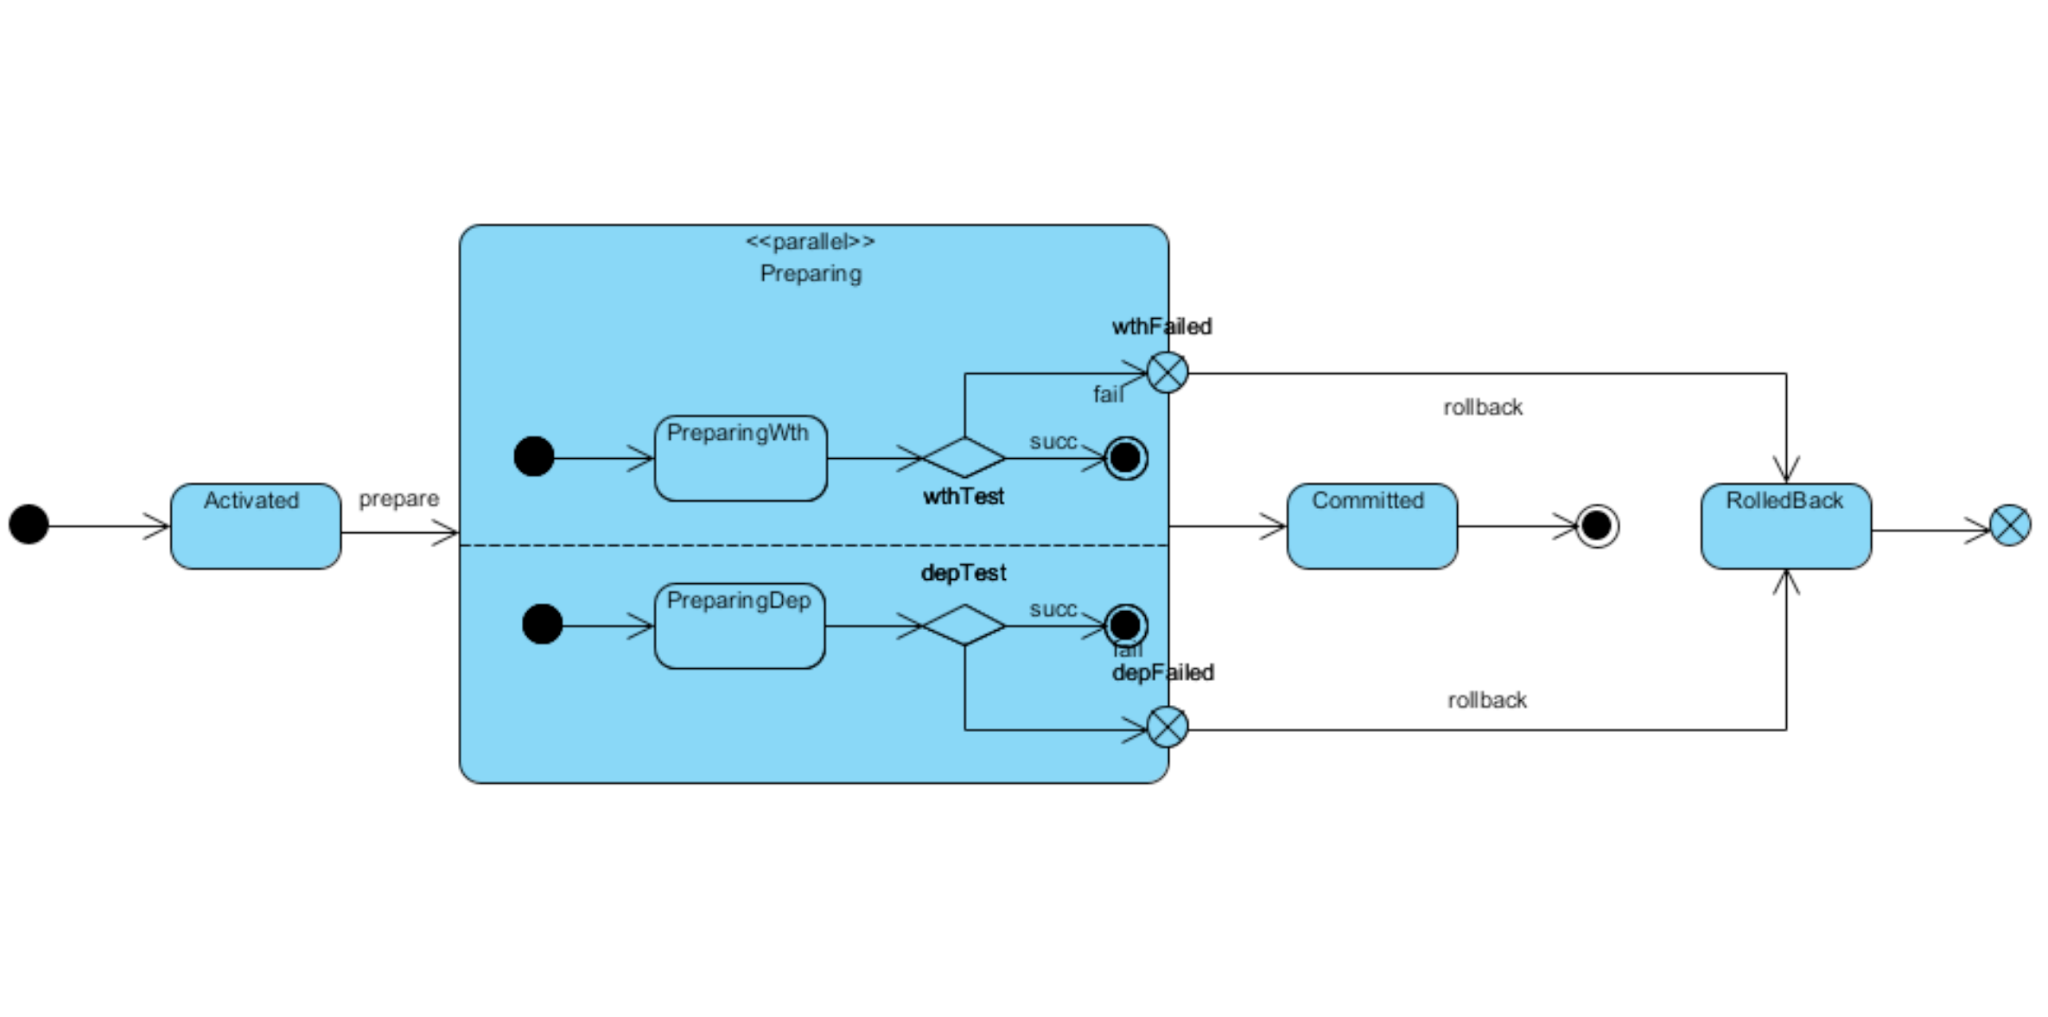
\includegraphics[width=0.9\textwidth]{FSM-hw.png}
\caption{Original FSM with Composite States}
\label{fig:fsm-original}
\end{figure}

The original finite state machine represents the starting point of our analysis. This diagram contains composite states that encapsulate multiple sub-states and transitions within a single high-level state. The composite state approach provides hierarchical organization and allows for complex state relationships.

The original FSM serves as the foundation for understanding the business logic that needs to be preserved while transforming the execution model. It demonstrates the natural grouping of related operations and establishes the baseline behavior that both the flattened and parallel versions must maintain.

\section*{FSM-Flat: Sequential Execution Model}

\begin{figure}[H]
\centering
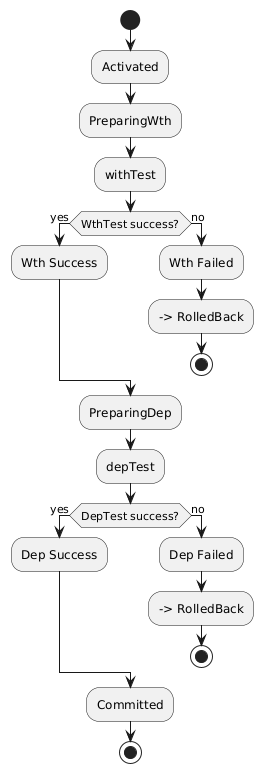
\includegraphics[width=0.35\textwidth]{FSM-flat.png}
\caption{Flattened Sequential Execution Model}
\label{fig:fsm-flat}
\end{figure}

The FSM-flat diagram implements a sequential execution pattern where operations are performed one after another in a predefined order. This model represents the "flattened" version of the original composite states, eliminating hierarchical nesting while preserving the logical flow.

\subsection*{Process Flow Analysis}

The system begins in an \texttt{Activated} state and immediately proceeds to prepare for withdrawal processing. During the \texttt{PreparingWth} phase, the system sets up the necessary conditions for executing a withdrawal test. The \texttt{withTest} operation is then performed to validate the withdrawal functionality.

Upon completion of the withdrawal test, the system evaluates the results through a decision point. If the withdrawal test succeeds, the process moves to the \texttt{Wth Success} state and continues to the next phase. However, if the test fails, the system transitions to a \texttt{Wth Failed} state and immediately proceeds to rollback operations before terminating the entire process.

Assuming the withdrawal test passes, the system then moves to the deposit processing phase. It enters the \texttt{PreparingDep} state to prepare for deposit operations, followed by executing the \texttt{depTest} operation. Similar to the withdrawal phase, the system evaluates the deposit test results at a decision point.

If the deposit test succeeds, the process reaches the \texttt{Dep Success} state and proceeds to the final \texttt{Committed} state, indicating successful completion of both operations. If the deposit test fails, the system enters the \texttt{Dep Failed} state and performs rollback operations before terminating.

\newpage
\section*{FSM-Fork-Join: Parallel Execution Model}

\begin{figure}[H]
\centering
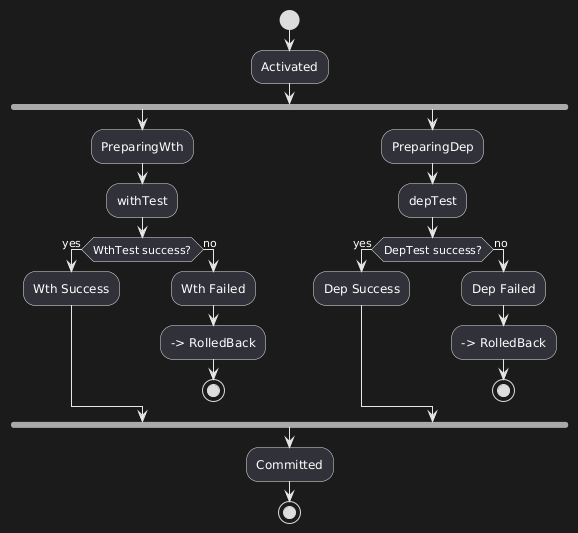
\includegraphics[width=0.8\textwidth]{FSM-fork-join.png}
\caption{Parallel Execution Model with Fork-Join}
\label{fig:fsm-fork-join}
\end{figure}

The FSM-fork-join diagram implements a parallel execution pattern where operations can be performed concurrently, potentially improving system efficiency and reducing overall processing time.

\subsection*{Parallel Process Flow Analysis}

The process begins identically with an \texttt{Activated} state, but immediately after activation, the workflow splits into two parallel branches using a fork construct. This allows both withdrawal and deposit operations to be prepared and tested simultaneously.

The first parallel branch handles withdrawal processing. It follows the same logical sequence as the sequential model: \texttt{PreparingWth}, \texttt{withTest} execution, and result evaluation. Success leads to \texttt{Wth Success}, while failure results in \texttt{Wth Failed} state and rollback termination.

The second parallel branch independently handles deposit processing. It mirrors the withdrawal branch with \texttt{PreparingDep}, \texttt{depTest} execution, and result evaluation, leading to either \texttt{Dep Success} or \texttt{Dep Failed} states with appropriate rollback handling.

The critical difference lies in the synchronization point after both parallel branches. The join construct ensures that both withdrawal and deposit operations must complete successfully before the process can advance to the \texttt{Committed} state. If either branch fails and triggers a rollback, the entire process terminates without reaching the final state.

\newpage
\section*{Comparative Analysis}

\subsection*{Execution Patterns and Performance}

The fundamental distinction between these models lies in their approach to concurrency and execution efficiency. The sequential model processes operations in a strict order, ensuring that withdrawal operations complete entirely before deposit operations begin. This approach provides predictable timing and simpler error handling but may result in longer overall execution times.

The parallel model allows simultaneous execution of both operation types, potentially reducing total processing time when operations are independent and can benefit from concurrent execution. However, this approach introduces complexity in synchronization and requires careful coordination to ensure both branches complete successfully.

\subsection*{System Design Implications}

From a system design perspective, the sequential model offers easier debugging and more straightforward error tracing since the execution path is linear. The parallel model provides better resource utilization and performance benefits but requires more sophisticated error handling and state management mechanisms.

The flattened sequential model eliminates the hierarchical complexity of composite states while maintaining a clear, linear execution path. This makes it easier to understand and maintain compared to the original composite state design.

\subsection*{Error Handling and Rollback Mechanisms}

Both models implement robust error handling with rollback capabilities. In the sequential model, rollback is straightforward since operations occur in sequence. The parallel model requires more complex rollback coordination, as failure in either branch must properly terminate both parallel execution paths.

\subsection*{Use Case Recommendations}

The choice between these patterns depends on specific system requirements:

\begin{itemize}
  \item \textbf{Sequential execution} is preferred when operations have dependencies, when system simplicity is prioritized, or when debugging and maintenance are critical concerns
  \item \textbf{Parallel execution} is beneficial when operations are independent, when performance optimization is critical, and when the system can handle the additional complexity of concurrent execution management
  \item \textbf{Original composite states} provide good organization for complex hierarchical behaviors but may be overkill for simple sequential processes
\end{itemize}

\section*{Conclusion}

This analysis demonstrates three different approaches to modeling the same business process using UML activity diagrams. The transformation from composite states to both sequential and parallel execution models shows how the same logical requirements can be implemented using different execution strategies.

The flattened sequential model successfully eliminates the complexity of composite states while maintaining clear, linear execution. The parallel fork-join model offers potential performance improvements through concurrent execution but introduces additional complexity in synchronization and error handling.

Each approach has its merits and should be chosen based on specific system requirements, including performance constraints, resource availability, error handling complexity, and the independence of the operations being performed. The key insight is that proper modeling allows for flexible implementation strategies while preserving the core business logic and ensuring system reliability.

\end{document}
